\section{A Metaprogramming Approach}
\label{Ch5:Sec:Meta}

\begin{comment}
Begin by saying a few words about what metaprogramming is. Then go into subsections. Idea:
1. Establish difficulty of doing computations in \C. Give examples, yes, but also stress that existing automation was unable to unpack the structural nuances of the way \C is defined. Also maybe talk about the whole "is I a numeral" debate, but I think this might be a rabbit-hole...
2. Talk about the algorithm behind norm_numI. Talk about the original version we worked on with Heather and Edison at/after metaprogramming and at Xena.
3. Say something about what Heather's latest modifications look like. Maybe also talk about how the approach can be generalised to quaternion algebras or splitting fields (what's similar and what's different between norm_numI and these things), but don't talk about the maths of either of these. Stress that this is still under development, and that this opens the door to a world of metaprogramming possibilities.
\end{comment}

The formalisation of the solution to the sphere packing problem brought to light a longstanding difficulty faced by the Lean community: a lack of automation for performing computations in $\C$. After a discussion with Heather Macbeth, who is experienced in creating automation for Lean, the author and Xie, with Macbeth's guidance and Mehta's invaluable inputs, embarked on the development of a normalisation-simplification automation procedure for performing computations in $\C$.

% I will condense the stuff below in the shorter (for-submission) version of this thesis. I'll leave it as is over here though... maybe this will come in handy someday...

Lean, like other interactive theorem provers, primarily interacts with its users through \textbf{tactics}. Fundamentally, the proof of a theorem in Lean is given by a \textbf{proof term}, which can be thought of as a concise expression that captures the information of how the hypotheses or inputs of the theorem are transformed into its conclusion by giving exactly the conclusion into which these inputs are transformed. A tactic is a command that, when invoked by a Lean user, performs a step in the construction of the proof term for a theorem.

The most basic tactics can be thought of as being `syntax sugar' rather than invocations of computation or reasoning algorithms. Consider the following code.
% MORE LATEX ERRORS! GAHHHHHHHH
\begin{lstlisting}[caption=A tactic-mode proof of the associativity of $\land$, label=Ch5:Listing:And_assoc_tactic]
example (P Q R : Prop) : P ∧ (Q ∧ R) → (P ∧ Q) ∧ R := by
  intro h
  constructor
  · constructor
    · exact h.1
    · exact h.2.1
    · exact h.2.2
\end{lstlisting}

In this example, the \lstinline|constructor| tactic is syntax sugar for an \textit{anonymous constructor}; the \lstinline|intro| tactic is syntax sugar for the input of a function; and the \lstinline|exact| tactic is syntax sugar for placing an exact term at a specific point in the proof term.

There are more advanced tactics, however, that construct proof terms automatically. For instance, results in intuitionistic propositional logic, such as the associativity of $\land$, are handled by \lstinline|itauto|.

\begin{lstlisting}[caption=A one-line tactic proof for the associativity of $\land$, label=Ch5:Listing:And_assoc_itauto]
example (P Q R : Prop) : P ∧ (Q ∧ R) ↔ (P ∧ Q) ∧ R := by itauto
\end{lstlisting}

Such tactics have immense utility, resulting in shorter, more readable proofs and a speedier, less vexatious interactive theorem proving experience. The science of writing such tactics is called \textbf{metaprogramming}. Given how computationally involved the construction of Viazovska's Magic Function is (as seen in \Cref{Ch4:Chapter}), the author and Macbeth agreed, after a discussion, that the most efficient approach to formalising some of the computational aspects of Viazovska's argument was to write a tactic capable of handling them. Macbeth was running  a metaprogramming seminar at Imperial College London at the time, and after discussing the approaches such a tactic might use with Xie, Mehta and the author, she wrote skeleton code that the author and Xie filled in together. The result of this was \lstinline|norm_numI|. In the forthcoming subsections, we explore the motivations and techniques used to develop \lstinline|norm_numI|.

\subsection{Complex Computations are Complex}

Computations in general are quite challenging to perform in interactive theorem provers. This is because such languages are designed for \textit{proof} rather than \textit{computation}. Indeed, tactics that simplify goals do not do so merely by simplifying expressions: they construct proofs that the simplified expression is, indeed, equal to the original expression. Existing tactics like \lstinline|norm_num|, \lstinline|simp| and \lstinline|field_simp| do not always do this successfully when the expressions in question are in $\C$ because they are not designed to navigate its particularities of the field (such as $i\inv = -i = \bar{i}$). Our approach was to create an improvement on \lstinline|norm_num| designed to work in $\C$. The reason for choosing \lstinline|norm_num| is that it is currently designed to deal with \textit{numerals} in semirings.

\lstinline|norm_num| works best in $\N$, $\Z$ and $\Q$. For example, it handles the following.
\begin{lstlisting}[caption={\lstinline|norm_num| simplifying expressions in $\N$, $\Z$ and $\Q$}]
example : (1 : ℕ) + 2 + 3 + 4 = 10 := by norm_num
example : (-2 : ℚ) * (3 + 8/9) = -70/9 := by norm_num
example : (-9 : ℤ) + 5 * (6 - 20) = -79 := by norm_num
\end{lstlisting}
It is worth mentioning, however, that \lstinline|norm_num| often has difficulties in $\R$. This is due to the immense technical detail baked into the very definition of $\R$. For example, the following is not handled by \lstinline|norm_num|.

\begin{lstlisting}[caption=An expression in $\R$ not handled immediately by simplification tactics, label=Ch5:Listing:pi_sub_one_norm_num_fail]
example : (π - 1) / (π - 1) = 1 := by
  have h₁ : (1 : ℝ) < 3 := by norm_num
  have h₂ : 1 ≠ π := ne_of_lt <| h₁.trans pi_gt_three
  have h₃ : π - 1 ≠ 0 := sub_ne_zero_of_ne h₂.symm
  field_simp [h₃]
\end{lstlisting}

Observe, however, that \lstinline|norm_num| \textit{is} able to prove the inequality $1 < 3$ despite it being an expression in $\R$. The reason is that \lstinline|norm_num| can navigate the canonical inclusions from $\N$, $\Z$ and $\Q$ into $\R$, meaning that it can simplify expressions in $\R$ that come from expressions it can simplify in $\N$, $\Z$ or $\Q$.\footnote{We say \lstinline|norm_num| can handle coercions.} It cannot, however, show that $1 < \pi$, because it does not treat $\pi$ \textit{as a numeral}. In $\C$, \lstinline|norm_num| faces this challenge not only with real transcendental numbers like $\pi$ but also with the imaginary constant $i$. For instance, it does not handle the following.\footnote{Note that in Lean, the imaginary constant is denoted by an uppercase \lstinline|I| instead of a lowercase $i$. We will adhere to standard mathematical conventions and use a lowercase $i$ when referring to the imaginary constant in informal contexts.}

\begin{lstlisting}[caption={A nontrivial computation in $\C$, done formally}, label=Ch5:Listing:long_tactic_pf_example_complex]
example : (1 + I) * (1 + I * I * I) = 2 := by
  simp only [I_mul_I, neg_mul, one_mul, mul_add, mul_one, mul_neg, add_mul, neg_add_rev, neg_neg]
  ring
\end{lstlisting}

Observe that $\parenth{1 + i}\parenth{1 + i \cdot i \cdot i}$ lies in $\Z[i]$. This means that if it is expressed as $a + bi$, with $a$ and $b$ both being (not necessarily simplified) real expressions, then in fact, $a$ and $b$ are both images of expressions in $\Z$. This means that \lstinline|norm_num| would be able to individually handle both $a$ and $b$, resulting in a simplified expression of the form $a' + b'i$, with $a'$ and $b'$ being simplified. This suggests that the key to writing a tactic that can simplify expressions like those in \Cref{Ch5:Listing:long_tactic_pf_example_complex} is to find a way to separate them into their real and imaginary parts.

\subsection{Parsing and Normalisation}

The core idea behind \lstinline|norm_num| is simplifying expressions by computing normal forms. In its most basic form, \lstinline|norm_num| attempts to prove equalities of by putting the left and right hand sides in unique normal forms that can simply be inspected to check if the two sides are equal. As was motived above, the right target normal form for an expression in $\C$ is splitting it into its real and imaginary parts, both of which are real expressions, and normalising them as much as possible.

The key to \lstinline|norm_numI| is the \href{https://github.com/thefundamentaltheor3m/Sphere-Packing-Lean/blob/05f51ee8f61972da1b0a5ee360c4c57c1b599cca/SpherePacking/Tactic/NormNumI.lean#L72}{\lstinline|parse| function}. It separates an expression $z \in \C$ into its real and imaginary parts by performing a recursive pattern-match. For example, if the outermost operation is addition---ie, if $z = z_1 + z_2$---then it calls itself on both $z_j$, obtaining real and imaginary parts $a_j, b_j \in \R$ and proofs that $z_j = a_j + b_ji$, and returns the expression $\parenth{a_1 + a_2} + \parenth{b_1 + b_2}i$ as well as a proof that $z = \parenth{a_1 + a_2} + \parenth{b_1 + b_2}i$, which it obtains via a helper lemma \href{https://github.com/thefundamentaltheor3m/Sphere-Packing-Lean/blob/05f51ee8f61972da1b0a5ee360c4c57c1b599cca/SpherePacking/Tactic/NormNumI.lean#L20}{\lstinline|split_add|}. It performs similar recursive actions if $z$ is of the form $z_1 \cdot z_2$, $z_1\inv$, $z_1 / z_2$, $-z_1$, $z_1 - z_2$, $\overline{z_1}$, $z_1^n$ for some $n \in \N$, $i$, or a decimal/natural number. The recursion is guaranteed to terminate, because an expression that is fed into the function cannot contain infinitely many characters.

\begin{boxexample}\label{Ch5:Eg:Parse}
    The expression $z = \parenth{1 + i}\parenth{1 + i \cdot i \cdot i}$ (cf. \Cref{Ch5:Listing:long_tactic_pf_example_complex}) would be parsed in the following manner.
    \begin{enumerate}[noitemsep]
        \item To parse $z$, write $z = z_1 \cdot z_2$, where $z_1 = 1 + i$ and $z_2 = 1 + i \cdot i \cdot i$.
        \item To parse $z_1$, write $z_1 = z_{11} + z_{12}$ where $z_{11} = 1$ and $z_{12} = i$.
        \item $z_{11}$ is parsed as $1 + 0i$.
        \item $z_{12}$ is parsed as $0 + 1i$.
        \item By \lstinline|split_add|, $z_1 = z_{11} + z_{12}$ is parsed as
              \begin{align*}
                  \parenth{1 + 0} + \parenth{0 + 1}i
              \end{align*}
        \item To parse $z_2$, write $z_2 = z_{21} + z_{22}$, where $z_{21} = 1$ and $z_{22} = i \cdot i \cdot i$.
        \item $z_{21}$ is parsed as $1 + 0i$.
        \item To parse $z_{22}$, write $z_{22} = z_{221} \cdot z_{222}$, where $z_{221} = i \cdot i$ and $z_{222} = i$.
        \item To parse $z_{221}$, write $z_{221} = z_{2211} \cdot z_{2212}$, where $z_{2211} = i$ and $z_{2212} = i$.
        \item $z_{2211}$ is parsed as $0 + 1i$.
        \item $z_{2212}$ is parsed as $0 + 1i$.
        \item By \lstinline|split_mul|, $z_{221} = z_{2211} \cdot z_{2212}$ is parsed as
              \begin{align*}
                  \parenth{0 \cdot 0 - 1 \cdot 1} + \parenth{0 \cdot 1 + 0 \cdot 1}i
              \end{align*}
        \item $z_{222}$ is parsed as $0 + 1i$.
        \item By \lstinline|split_mul|, $z_{22} = z_{221} \cdot z_{222}$ is parsed as
              \begin{align*}
                  \parenth{
                    \parenth{0 \cdot 0 - 1 \cdot 1}
                        \cdot
                    0
                    -
                    \parenth{0 \cdot 1 + 1 \cdot 0}
                        \cdot
                    1
                  } + \parenth{
                    \parenth{0 \cdot 0 - 1 \cdot 1}
                        \cdot
                    1
                    +
                    0
                        \cdot
                    \parenth{0 \cdot 1 + 1 \cdot 0}
                  }i
              \end{align*}
        \item By \lstinline|split_add|, $z_2 = z_{21} + z_{22}$ is parsed as
              \begin{align*}
                  &\parenth{1 + \parenth{
                    \parenth{0 \cdot 0 - 1 \cdot 1}
                        \cdot
                    0
                    -
                    \parenth{0 \cdot 1 + 1 \cdot 0}
                        \cdot
                    1
                  }} \\
                  + &\parenth{0 + \parenth{
                    \parenth{0 \cdot 0 - 1 \cdot 1}
                        \cdot
                    1
                    +
                    0
                        \cdot
                    \parenth{0 \cdot 1 + 1 \cdot 0}
                  }}i
              \end{align*}
        \item By \lstinline|split_mul|, $z = z_1 + z_2$ is parsed as
              \hspace{-2em}
              \begin{align*}
                  &\Big(
                    \parenth{1 + 0}
                        \cdot
                    \parenth{1 + \parenth{
                        \parenth{0 \cdot 0 - 1 \cdot 1}
                            \cdot
                        0
                        -
                        \parenth{0 \cdot 1 + 1 \cdot 0}
                            \cdot
                        1
                    }} \\
                    & -
                    \parenth{0 + 1}
                        \cdot
                    \parenth{0 + \parenth{
                        \parenth{0 \cdot 0 - 1 \cdot 1}
                            \cdot
                        1
                        +
                        0
                            \cdot
                        \parenth{0 \cdot 1 + 1 \cdot 0}
                    }}
                  \Big) \\
                  + &\Big(
                    \parenth{1 + 0}
                        \cdot
                    \parenth{0 + \parenth{
                        \parenth{0 \cdot 0 - 1 \cdot 1}
                            \cdot
                        1
                        +
                        0
                            \cdot
                        \parenth{0 \cdot 1 + 1 \cdot 0}
                    }} \\
                    & +
                    \parenth{1 + \parenth{
                        \parenth{0 \cdot 0 - 1 \cdot 1}
                            \cdot
                        0
                        -
                        \parenth{0 \cdot 1 + 1 \cdot 0}
                            \cdot
                        1
                    }}
                        \cdot
                    \parenth{0 + 1}
                  \Big)i
              \end{align*}
    \end{enumerate}
\end{boxexample}

\begin{wrapfigure}{r}{0.4\linewidth}
    \centering
    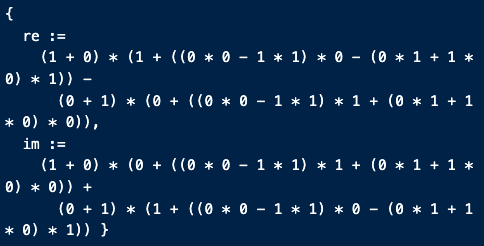
\includegraphics[width=0.95\linewidth]{Chapters/5_Lean/Images/norm_numI_parse_output.png}
    \caption{The Lean output of the steps shown in \Cref{Ch5:Eg:Parse}.}
    \label{Ch5:Fig:Parse_Example}
\end{wrapfigure}

Clearly, despite being mathematically valid, the result of parsing can be long and uninformative, making it an unsuitable choice of normal form for our purposes. However, by separating complex expressions into their real and imaginary parts, \lstinline|parse| perfectly sets us up to use an existing, highly effective normalisation procedure: \lstinline|norm_num| itself. Since \lstinline|parse| expresses any complex expression as a combination of two real expressions, the normalisation procedure simply makes calls to \lstinline|norm_num| to express each of them in a \textit{real} normal form. The result is a complex number in a normal form $a + bi$ (or, in Lean notation, \lstinline|{re := a, im := b}|) with $a$ and $b$ both simplified to the greatest extent possible (as expressions in $\R$) by applying \lstinline|norm_num|.

\lstinline|norm_numI| is currently implemented as a \lstinline|conv| tactic rather than a full tactic, meaning that it is only capable of modifying expressions and providing a proof that the modification is valid. It is not currently capable of proving goals, which are necessarily logical statements, such as equalities. It can be used as follows.

% Why is there an error in the following listing?
% Uncomment before submitting. Keep commented till then so easier to keep track of errors.
\begin{lstlisting}[caption={Using \lstinline|norm_numI| as a \lstinline|conv| tactic}, label=Ch5:Listing:norm_numI_as_conv]
example : (1 + I) * (1 + I * I * I) = 2 := by
  conv_lhs => norm_numI
  conv_rhs => norm_numI
\end{lstlisting}

After Macbeth, Xie and the author's initial success with this \lstinline|conv| tactic, Macbeth created an \textit{extension} of the existing \lstinline|norm_num| tactic that uses the parsing technique outlined above to handle complex expressions. This tactic is still being developed, but is being tested on active code from the project with immensely promising results.

% \subsection{Scope for Further Development}

% The benefits of having such a tactic cannot be overstated. There are numerous instances across the project where the collaborators have had to repeatedly prove computational facts in $\C$, such as $1 + i \neq 0$, or clear complex denominators to separate expressions into their real and imaginary parts. It is precisely this that motivated the development of \lstinline|norm_numI|, and indeed, \lstinline|norm_numI| is proving to be a viable solution.

% % Give an explicit example here from the repo

% The applicability of \lstinline|norm_numI|---or, at the very least, of the underlying idea, that the right normal form for expressions in $\C$ is to separate them into real and imaginary parts and express those in a normal form---extends well beyond expressions in $\C$. A key motivation for Xie, one of the co-creators of \lstinline|norm_numI| and an ardent algebraist, was to create a similar tactic that would normalise and simplify expressions in quaternion algebras. A discussion at a London Learning Lean event hosted at the London Institute of Mathematical Sciences in March 2025 sparked speculation among well-regarded members of the Lean Community that similar ideas might be applicable in other field extensions (with $\C$ regarded as $\quotient{\R[X]}{\parenth{X^2 + 1}}$ and $i$ as the image of $X$ via the quotient map). The idea would be that the separation into components corresponds to taking advantage of some linear independence criterion, with algebraic dependences not handled by the simplification step being captured by the helper lemmas in the normalisation step.

% There are numerous technical difficulties with implementing such a tactic that can work in other contexts, chief amongst them the fact that there would need to be a single modification to the tactic capable of handling very differently behaved algebraic structures (for instance, it would need to work the same way in quadratic, cubic, quartic and higher degree field extensions). It would hence need to have some awareness of the behaviours of each field in which it is applied, which is technically challenging. Nevertheless, the development of \lstinline|norm_numI| and the subsequent \lstinline|norm_num| modification marks a significant, and long overdue, step in the right direction, so that fewer nontrivial proofs are needed to prove trivial facts.